\documentclass[tikz,border=8pt]{standalone}
\usepackage[scaled=0.95]{helvet}
\renewcommand{\familydefault}{\sfdefault}
\usepackage[europeanresistors,americanvoltages]{circuitikz}
\definecolor{TEJNavy}{HTML}{1E2B55}
\definecolor{TEJBlue}{HTML}{1769AA}
\begin{document}
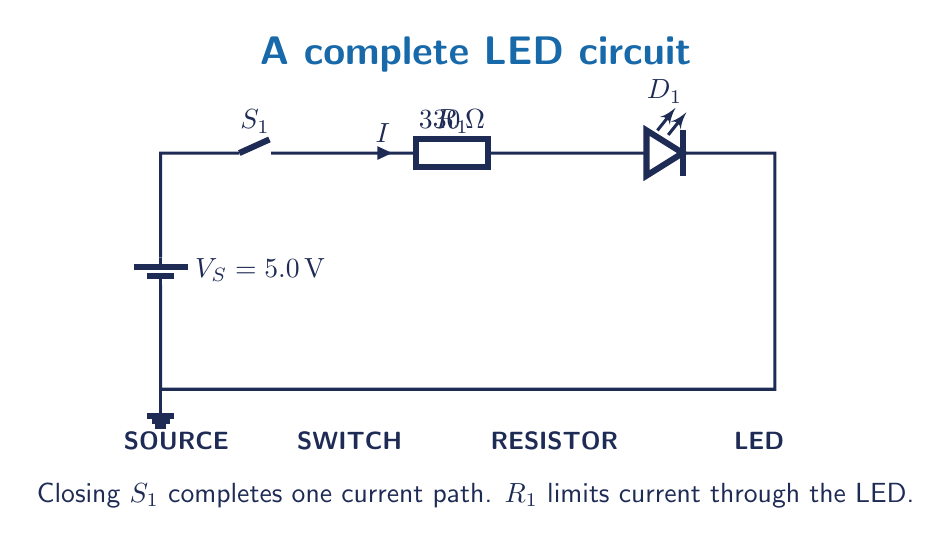
\begin{tikzpicture}[line width=1.1pt,draw=TEJNavy,text=TEJNavy,font=\sffamily]
  \ctikzset{bipoles/length=1.15cm}

  \node[font=\bfseries\Large,text=TEJBlue] at (4.0,4.25)
    {A complete LED circuit};
  \draw
    (0,0) node[ground] {}
    to[battery1,invert,l_={$V_S=5.0\,\mathrm{V}$}] (0,3)
    to[nos,l={$S_1$}] (2.4,3)
    to[R,l={$R_1$},a^={$330\,\Omega$},i>^={$I$}] (5.0,3)
    to[leD,l={$D_1$}] (7.8,3)
    -- (7.8,0) -- (0,0);
  \node[font=\bfseries\small,text=TEJNavy] at (0.2,-0.65) {SOURCE};
  \node[font=\bfseries\small,text=TEJNavy] at (2.4,-0.65) {SWITCH};
  \node[font=\bfseries\small,text=TEJNavy] at (5.0,-0.65) {RESISTOR};
  \node[font=\bfseries\small,text=TEJNavy] at (7.6,-0.65) {LED};
  \node[align=center] at (4.0,-1.35)
    {Closing $S_1$ completes one current path. $R_1$ limits current through the LED.};
\end{tikzpicture}
\end{document}
